\section{Componentes REAS del agente}
Los componentes REAS del agente son los siguientes:

\subsection{Rendimiento}
Para evaluar el rendimiento del agente, es suficiente con evaluar si cumple su meta, la cual consiste en recorrer indefinidamente los bordes interiores del ambiente. El agente también debe ser capaz de recorrer los pasillos estrechos (de 1 celda de tamaño) y, si este pasillo está bloqueado, volver por él hasta la salida.

\subsection{Entorno}
El agente tiene la siguiente información sobre el entorno:
\begin{itemize}
    \item El entorno es cuadriculado.
    \item El agente conoce la orientación del entorno (conoce donde se encuentra el \emph{Norte}, \emph{Este}, \emph{Sur} y \emph{Oeste} en cada momento).
    \item El agente sabe como realizar los movimientos en la dirección que ha decidido.
\end{itemize}

\subsection{Actuadores}

Los actuadores del agente son los 4 posibles movimientos hacia una casilla que se encuentra vacía:
\begin{itemize}
    \item \textbf{Norte}: avanzar hacia la casilla de arriba.
    \item \textbf{Este}: avanzar hacia la casilla de la derecha.
    \item \textbf{Sur}: avanzar hacia la casilla de abajo.
    \item \textbf{Oeste}: avanzar hacia la casilla de la izquierda.
\end{itemize}

\begin{figure}[!ht]
    \centering
    
\includegraphics[width=0.3\textwidth]{Movimientos}
    \caption{Actuadores del agente}
    \label{fig:actuadores}
\end{figure}

\FloatBarrier
\subsection{Sensores}
El agente puede percibir si las casillas \emph{Norte}, \emph{Este}, \emph{Sur} y \emph{Oeste} están libres u ocupadas. Así, el agente dispone de 4 entradas binarias, a las cuales se les asociará las variables \emph{$S_{1}$}, \emph{$S_{2}$}, \emph{$S_{3}$} y \emph{$S_{4}$} (el valor \emph{0} indicará que no hay pared y el valor \emph{1} indicará que sí hay pared).

\begin{figure}[!ht]
    \centering
    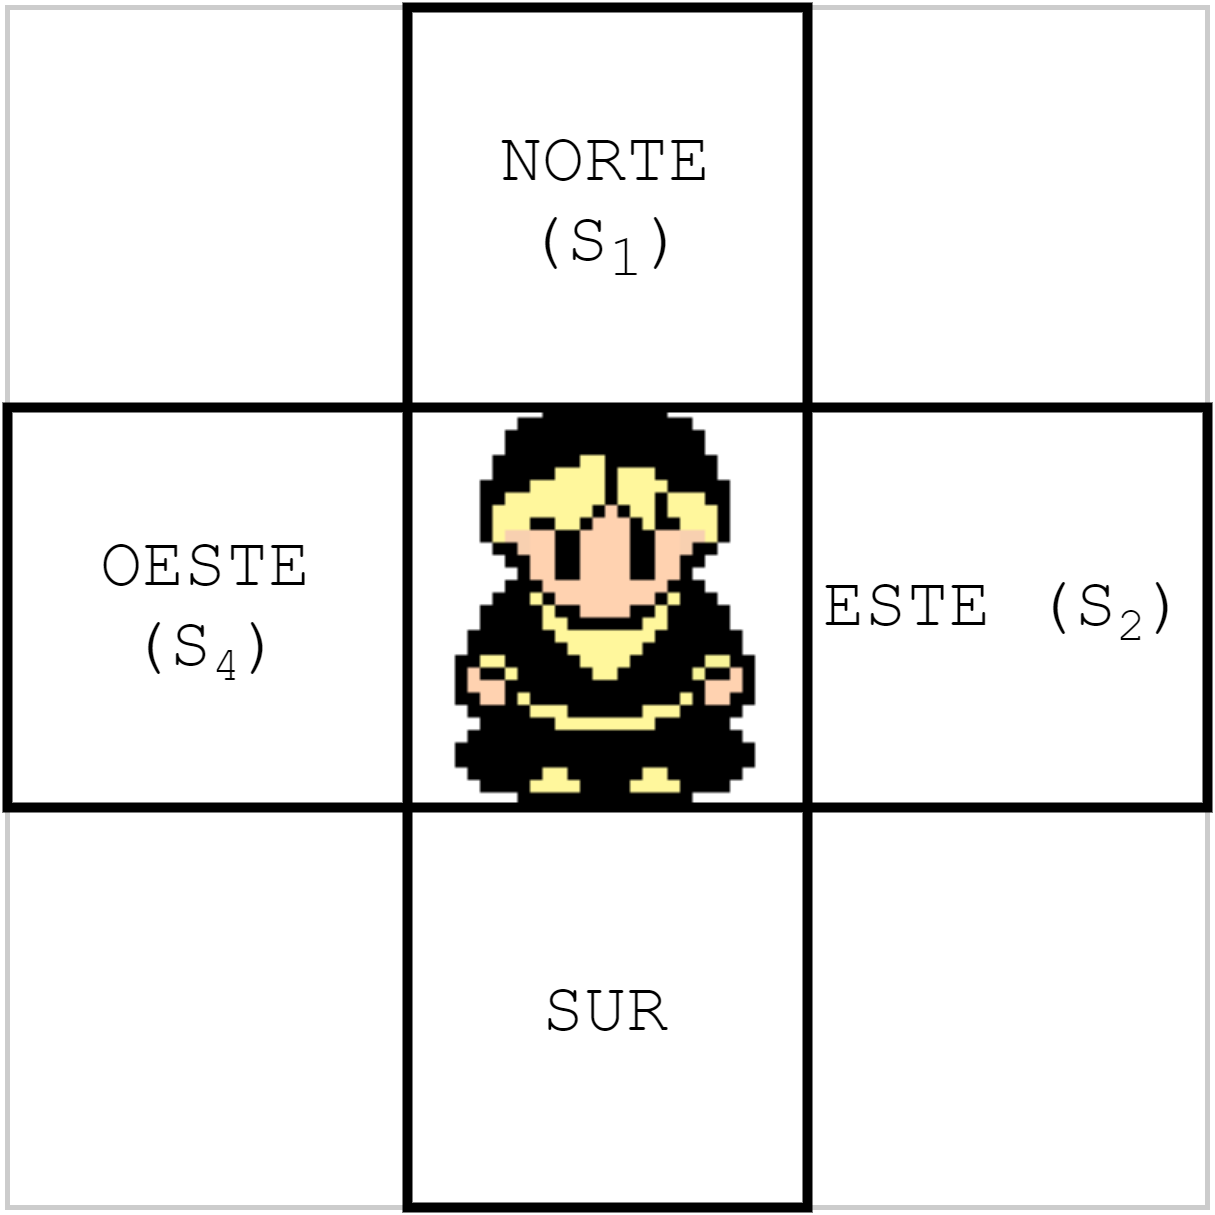
\includegraphics[width=0.3\textwidth]{Sensores}
    \caption{Sensores del agente}
    \label{fig:sensores}
\end{figure}

\section{Estado interno del agente}

Debido a que el agente está limitado a solo los 4 estímulos básicos, el agente necesita un estado interno para calcular correctamente la acción a realizar en cada situación. Este estado interno se compone de:

\begin{itemize}
    \item El vector de características actual y anterior. Al vector de características actual lo identificaremos como \emph{W} y al vector anterior como \emph{$W^{t-1}$}.
    \item La última acción realizada y la actual. La acción actual la identificaremos como \emph{A} y la anterior como \emph{$A^{t-1}$}
\end{itemize}

\section{Vector de características}

El vector de características constará de 8 componentes, las cuales indicarán si en las casillas que envuelven del agente hay una pared o no.

\begin{figure}[!ht]
    \centering
    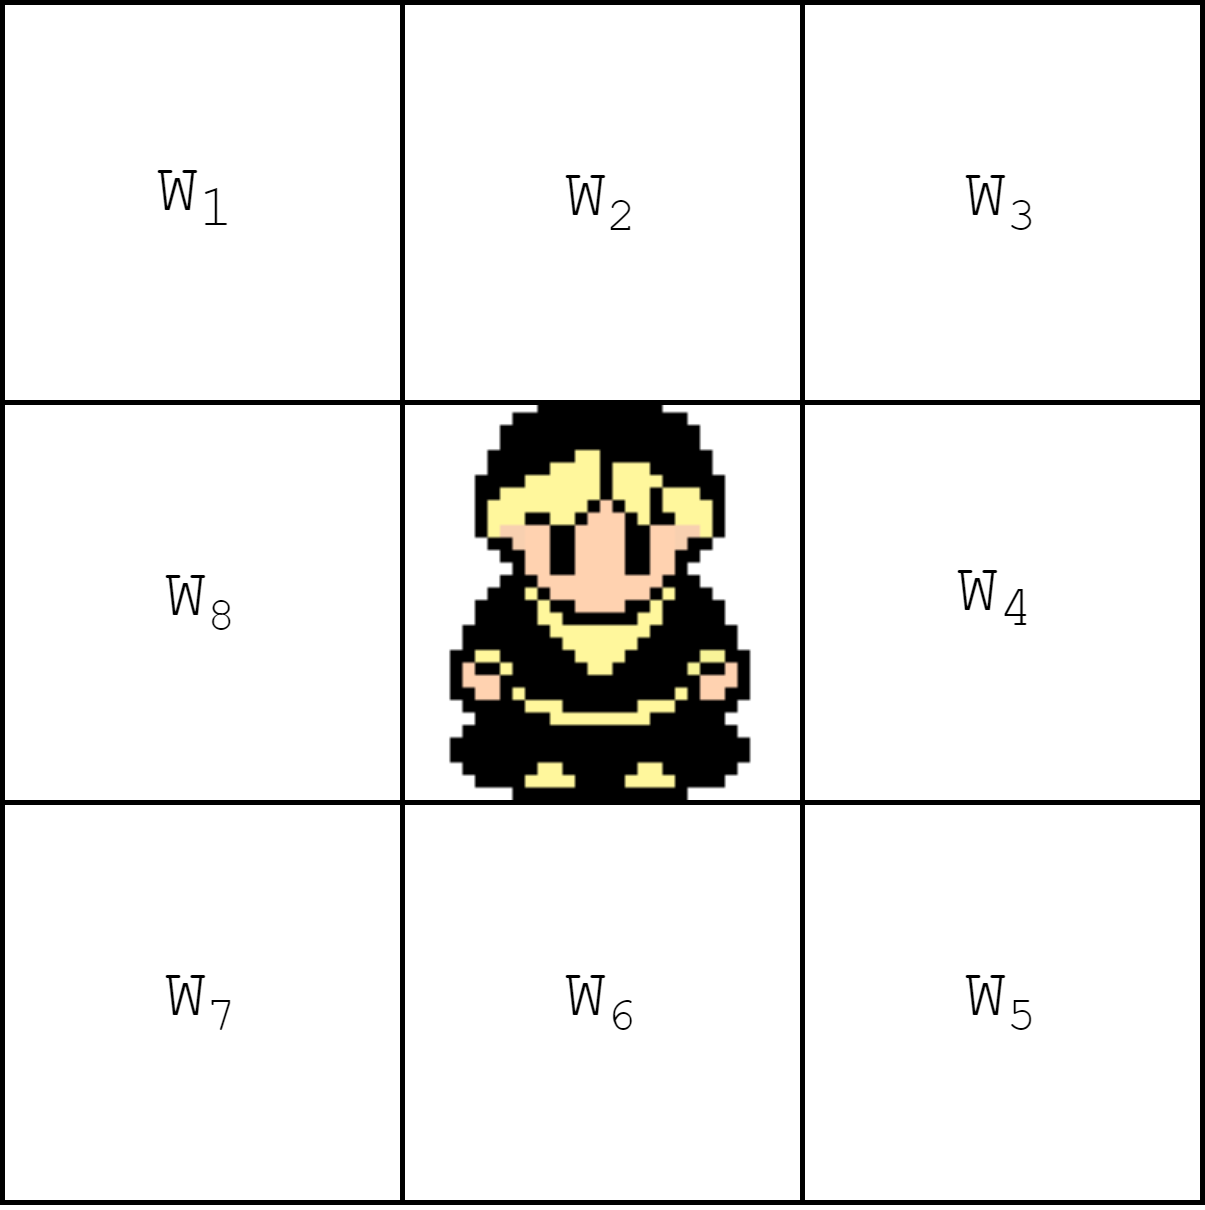
\includegraphics[width=0.3\textwidth]{Vector}
    \caption{Vector de características del agente}
    \label{fig:caracteristicas}
\end{figure}

Para calcular el vector de características necesitamos las entradas \emph{$S_{1}$}, \emph{$S_{2}$}, \emph{$S_{3}$} y \emph{$S_{4}$}. Estas entradas corresponderán a los valores \emph{$W_{2}$}, \emph{$W_{4}$}, \emph{$W_{6}$} y \emph{$W_{8}$} respectivamente. Estos valores no son suficientes para que el agente cumpla con su meta, así que también debemos calcular los valores de \emph{$W_{1}$}, \emph{$W_{3}$}, \emph{$W_{5}$} y \emph{$W_{7}$}. Para esto, se utilizará el vector de características anterior (\emph{$W^{t-1}$}) y la última acción ejecutada (\emph{$A^{t-1}$}). Así, el agente puede averiguar si hay una pared en estas variables de la siguiente forma:

\begin{itemize}
    \item \textbf{$W_{1}$}: si \emph{$W_{2}^{t-1}$} es verdadero y \emph{$A^{t-1} = Este$}.
    \item \textbf{$W_{2}$}: si \emph{$W_{4}^{t-1}$} es verdadero y \emph{$A^{t-1} = Sur$}.
    \item \textbf{$W_{3}$}: si \emph{$W_{6}^{t-1}$} es verdadero y \emph{$A^{t-1} = Oeste$}.
    \item \textbf{$W_{4}$}: si \emph{$W_{8}^{t-1}$} es verdadero y \emph{$A^{t-1} = Norte$}.
\end{itemize}

\begin{figure}[h]
\centering
    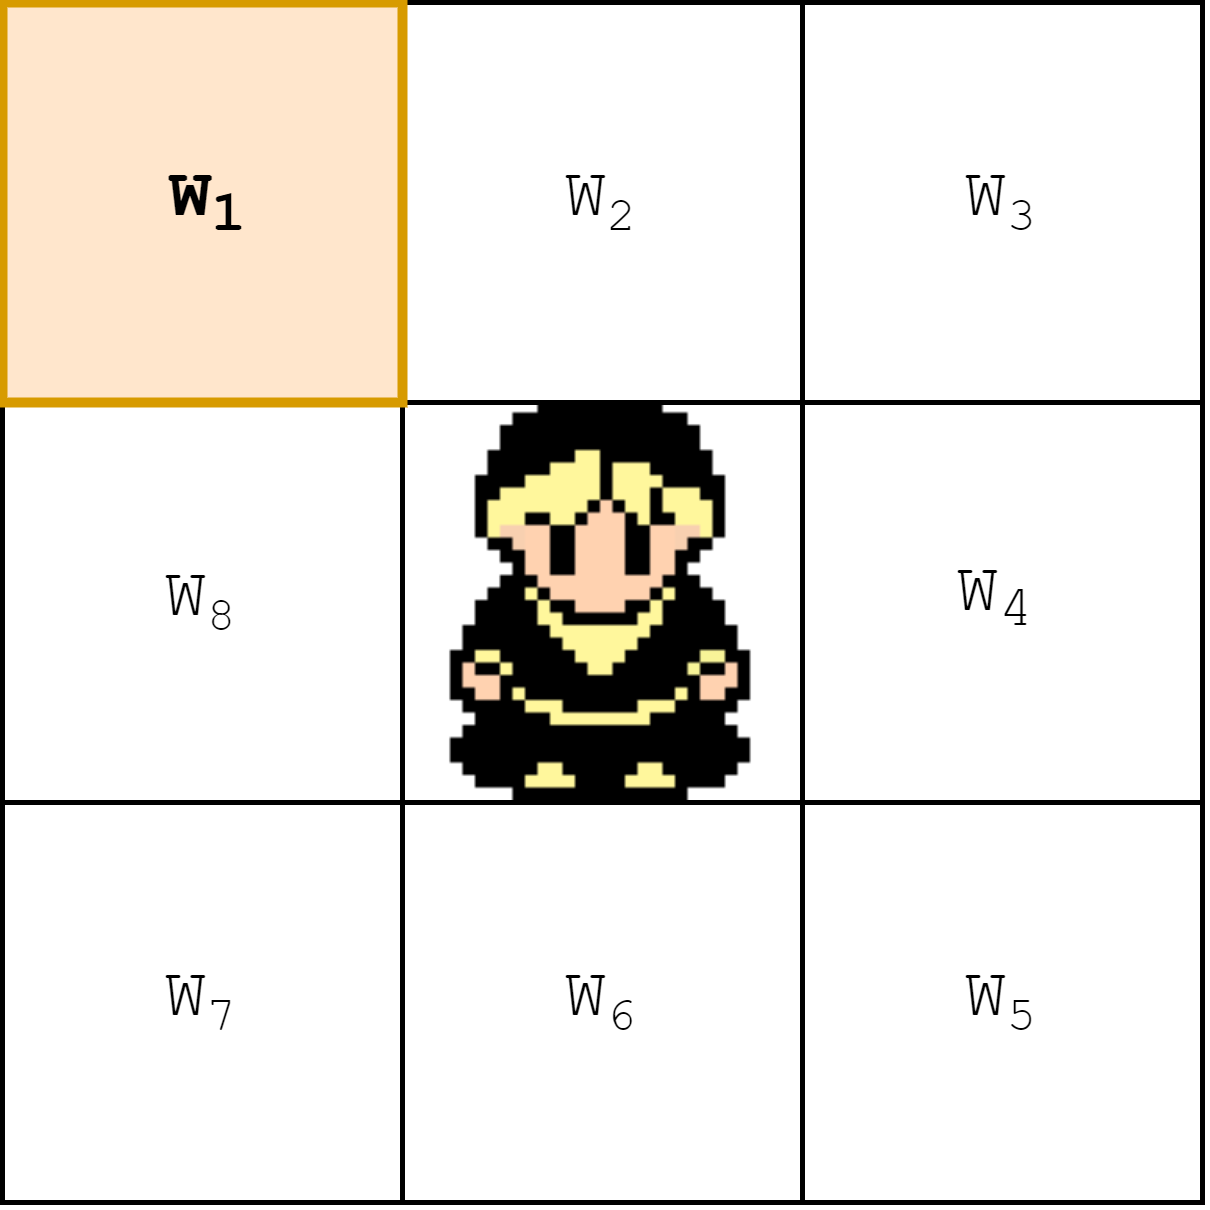
\includegraphics[width=.3\columnwidth]
        {W1}
    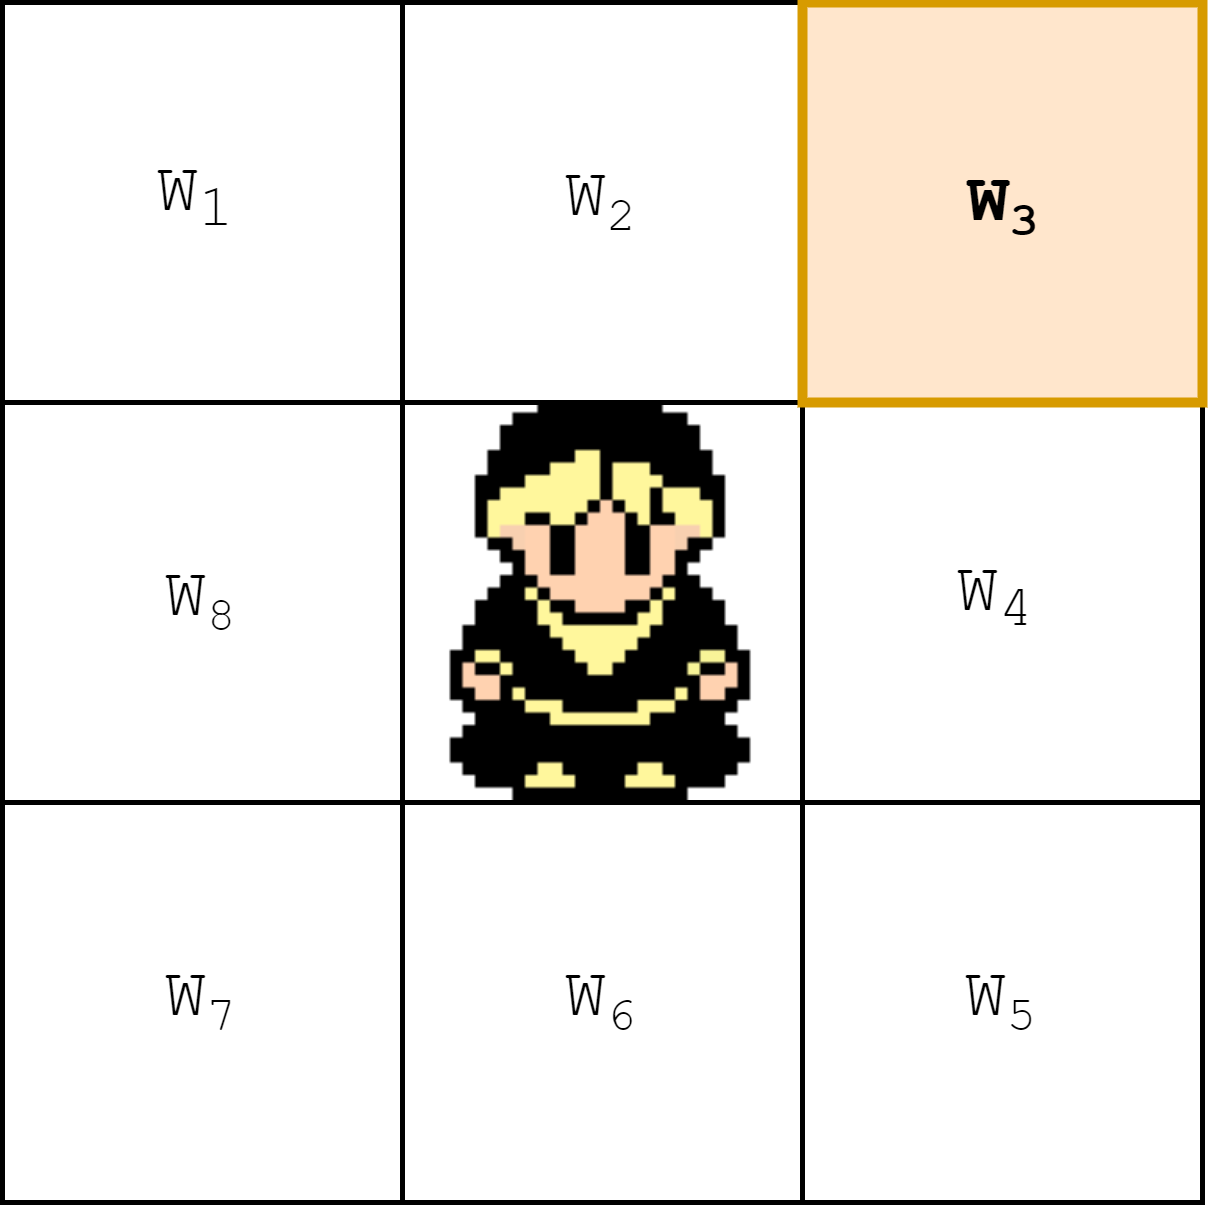
\includegraphics[width=.3\columnwidth]
        {W3}
    \\ %
    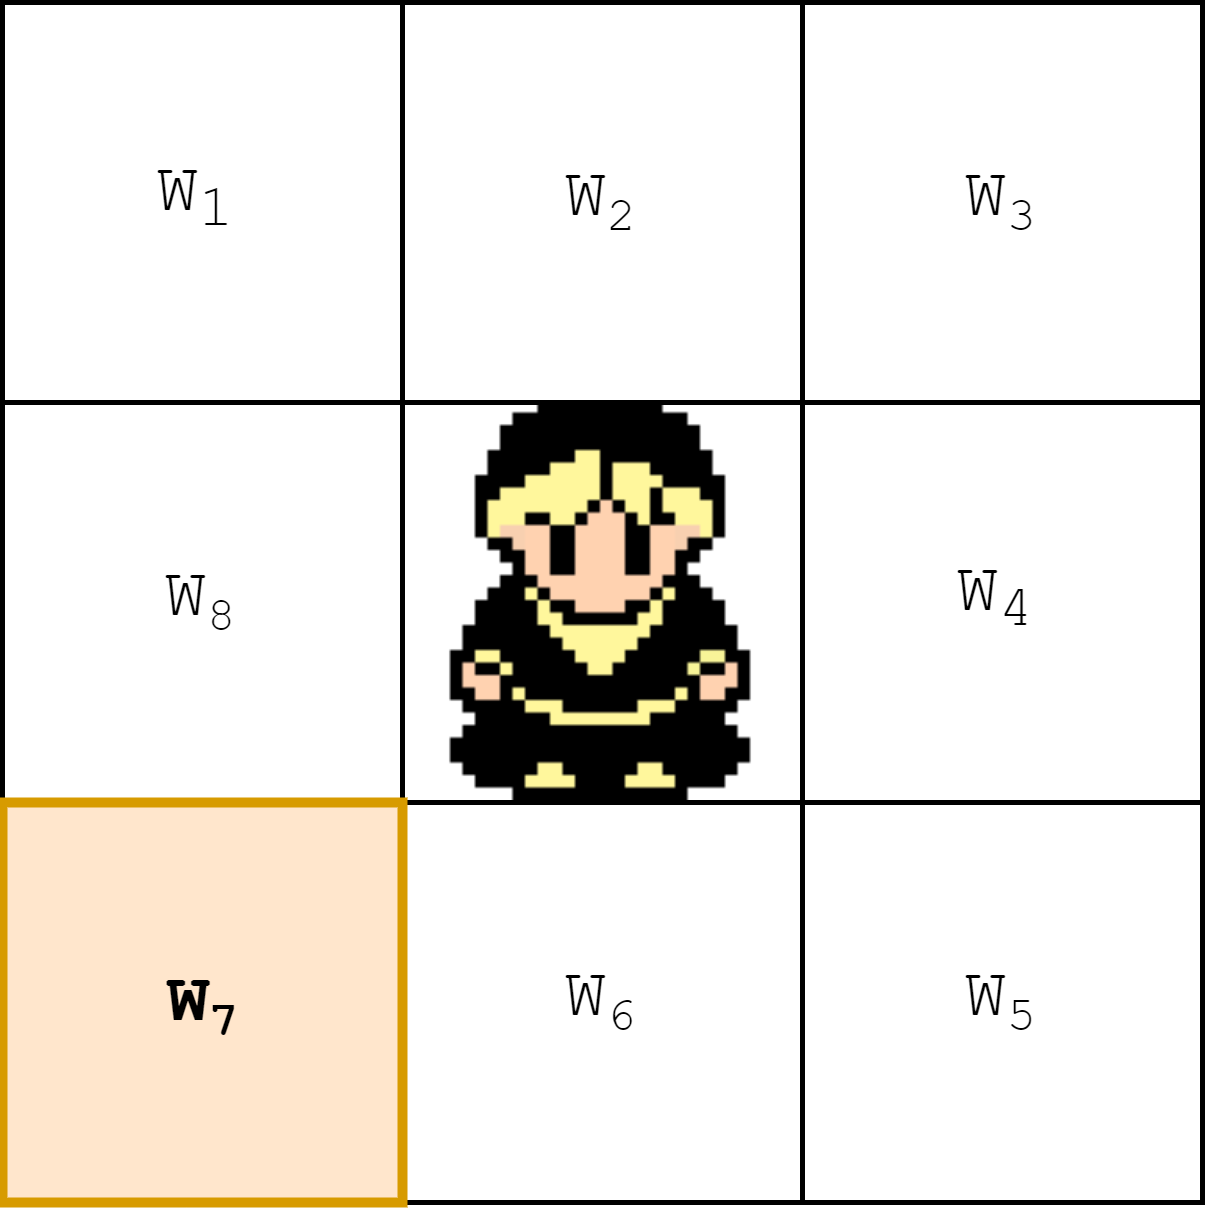
\includegraphics[width=.3\columnwidth]
        {W7}
    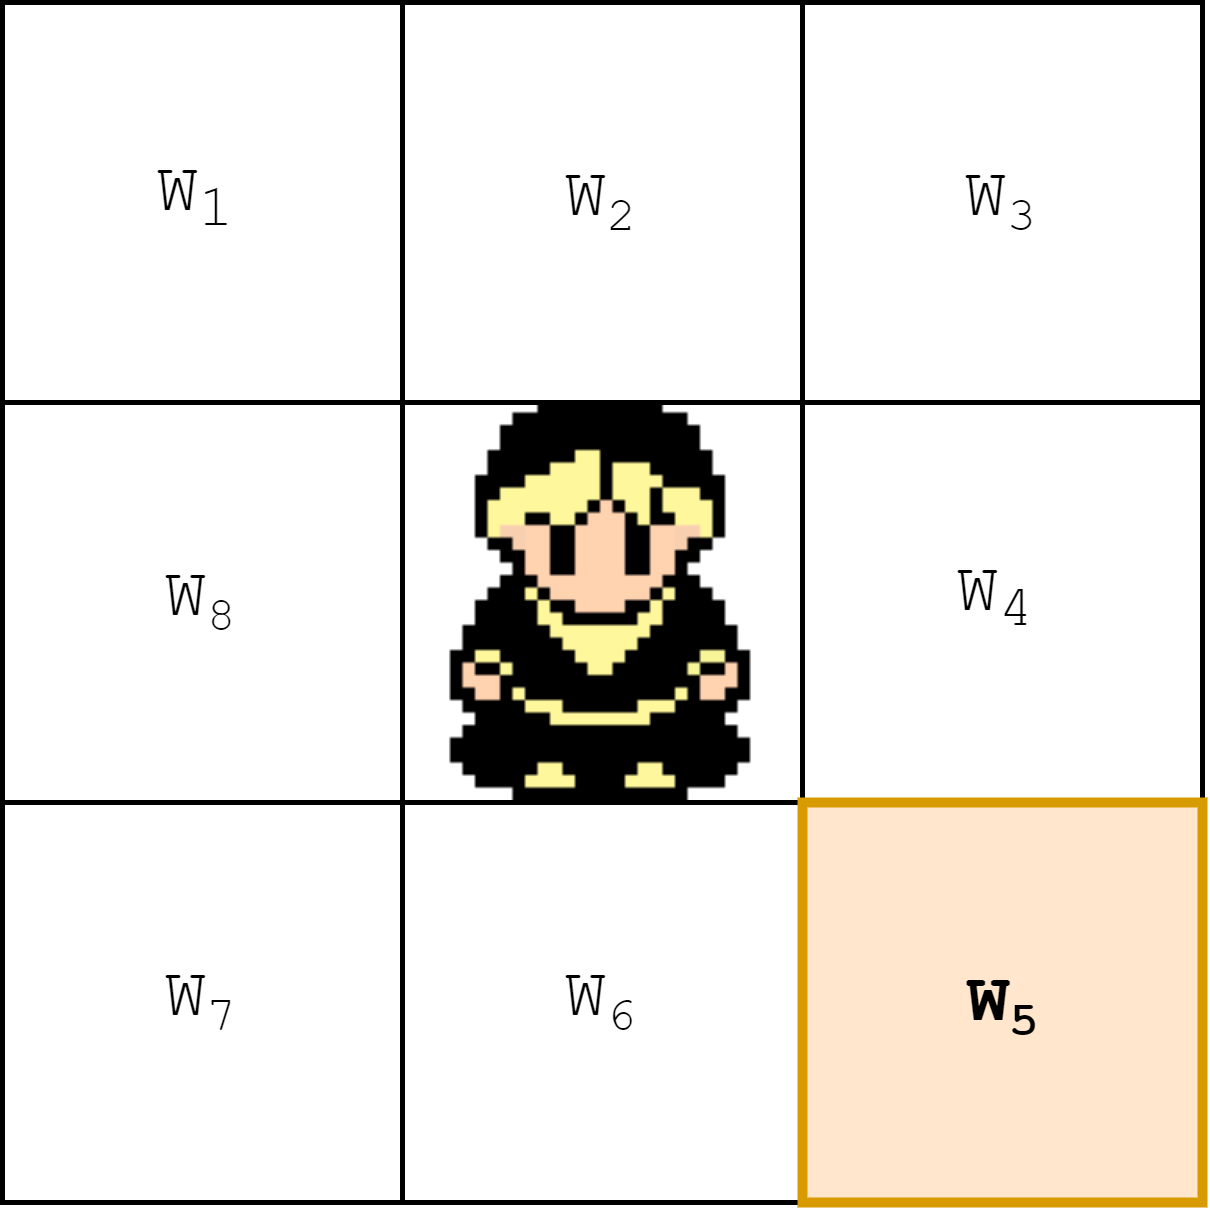
\includegraphics[width=.3\columnwidth]
        {W5}

  \caption{Estímulos que el agente no puede percibir}
\end{figure}

\FloatBarrier

\section{Base de reglas}
La base de reglas consiste en las reglas que utiliza el agente para moverse por el entorno. Estas reglas están ordenadas por una prioridad que está determinada según la situación en la que se encuentre el agente. Así, encontramos 3 categorías de reglas:

\subsection{Salida de un pasillo estrecho}
Son las reglas más prioritarias ya que indican al agente la acción que debe realizar cuando sale de un pasillo estrecho.

El agente determina que ha salido de un pasillo estrecho en los siguientes casos:
\begin{itemize}
    \item La acción anterior era \emph{Oeste} y sabe que en la casilla \emph{$W_{5}$} hay pared y en la casilla \emph{$W_{6}$} no hay pared (Figura 2.5 (a)). En este caso el agente sabrá que debe ir hacia el \emph{Sur}.
    
    \item La acción anterior era \emph{Sur} y sabe que en la casilla \emph{$W_{3}$} hay pared y en la casilla \emph{$W_{4}$} no hay pared  (Figura 2.5 (b)). En este caso el agente sabrá que debe ir hacia el \emph{Este}.
    
    \item La acción anterior era \emph{Este} y sabe que en la casilla \emph{$W_{1}$} hay pared y en la casilla \emph{$W_{2}$} no hay pared  (Figura 2.5 (c)). En este caso el agente sabrá que debe ir hacia el \emph{Norte}.
    
    \item La acción anterior era \emph{Norte} y sabe que en la casilla \emph{$W_{7}$} hay pared y en la casilla \emph{$W_{8}$} no hay pared  (Figura 2.5 (d)). En este caso el agente sabrá que debe ir hacia el \emph{Oeste}.
\end{itemize}

\begin{figure}[htb]
\centering
  \subfloat[Salida oeste]{%
    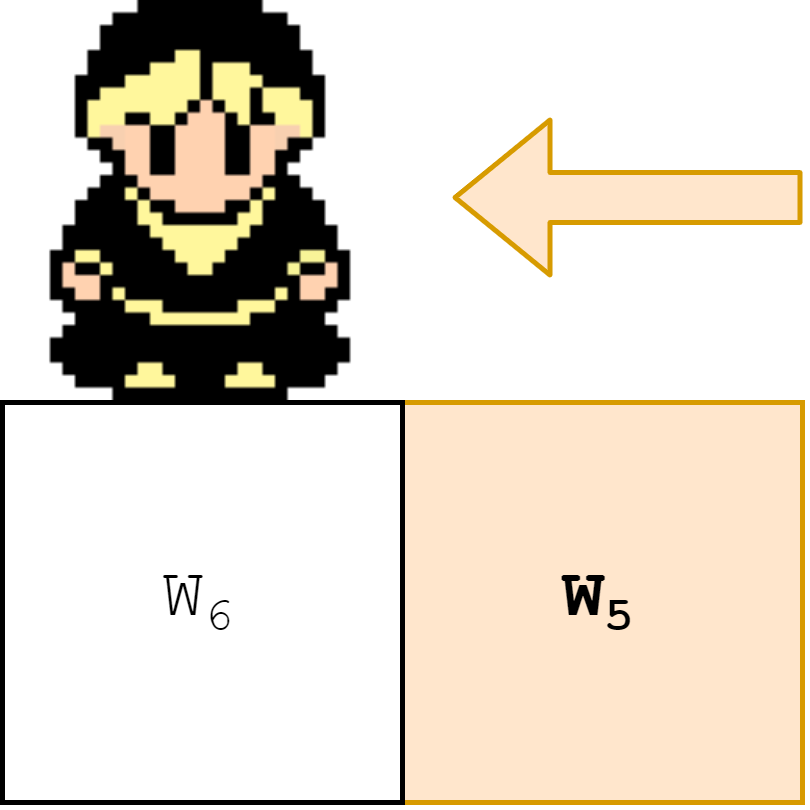
\includegraphics[width=.20\columnwidth]{salir_sud}}\hspace{1em}
  \subfloat[Salida sur]{%
    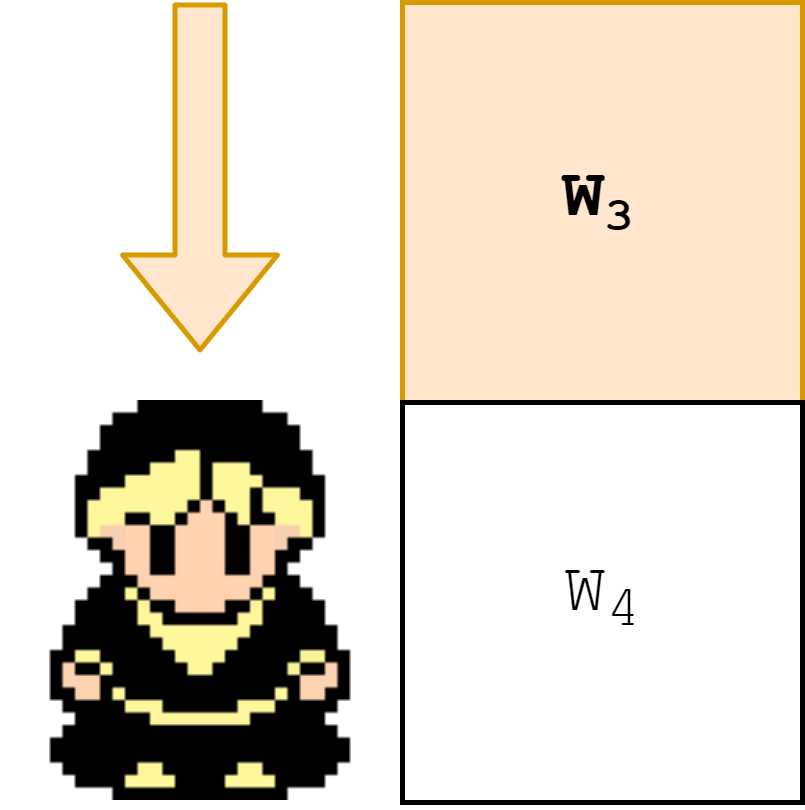
\includegraphics[width=.20\columnwidth]{salir_este}}\\
  \subfloat[Salida este]{%
    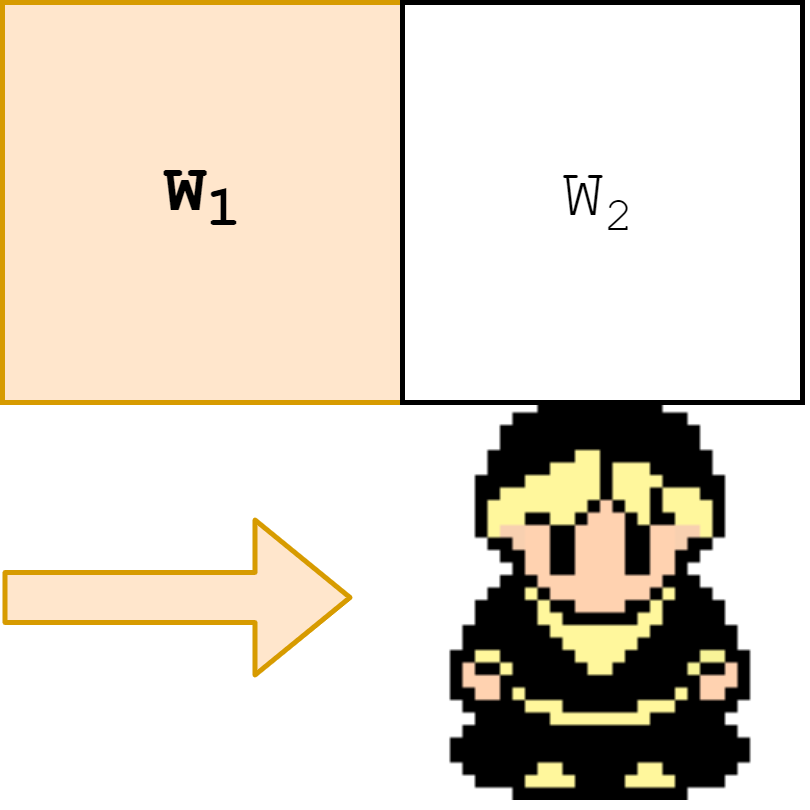
\includegraphics[width=.20\columnwidth]{salir_norte}}\hspace{1em}
  \subfloat[Salida norte]{%
    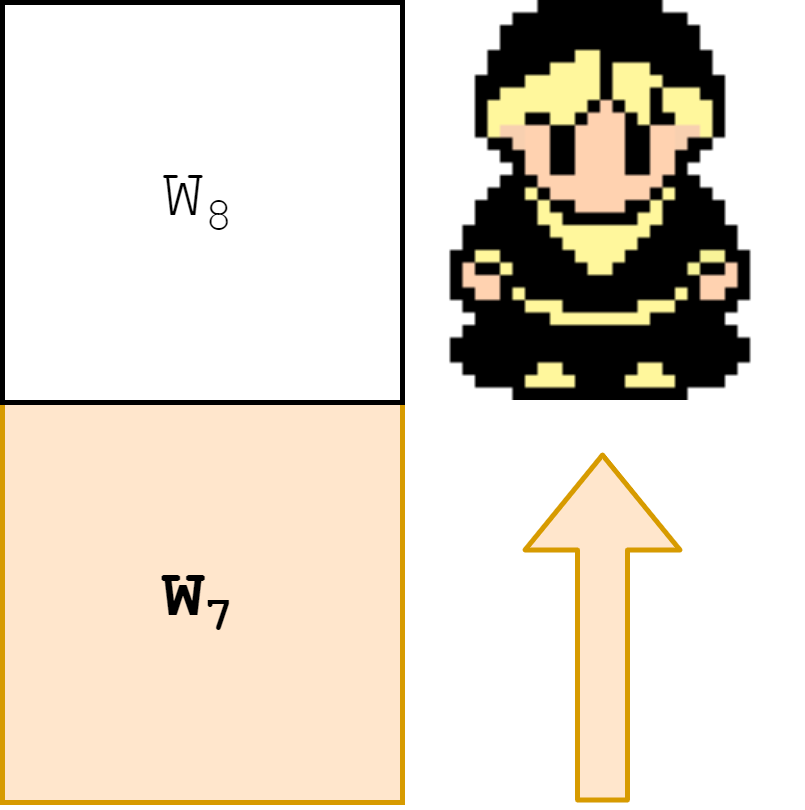
\includegraphics[width=.20\columnwidth]{salir_oeste}}
  \caption{Casos de salida de un pasillo estrecho}\label{fig:salir_pasillo}
\end{figure}

\FloatBarrier

\hfill

Con esta información, podemos establecer las siguientes reglas:

\begin{itemize}
    \item \emph{$A^{t-1} = Oeste \land W_{5} \land \neg W_{6} \longrightarrow A = Sur $}
    \item \emph{$A^{t-1} = Sur \land W_{3} \land \neg W_{4} \longrightarrow A = Este $}
    \item \emph{$A^{t-1} = Este \land W_{1} \land \neg W_{2} \longrightarrow A = Norte $}
    \item \emph{$A^{t-1} = Norte \land W_{7} \land \neg W_{8} \longrightarrow A = Oeste $}
\end{itemize}

Hay que destacar que esta reglas también están ordenadas según su prioridad de ejecución, ya que con este orden se consigue que el agente haga un recorrido en sentido antihorario.

\subsection{Recorrido de un pasillo estrecho}
Estás reglas van seguidas de las anteriores, ya que interesa que el agente salga de un pasillo (si es posible) a que esté recorriéndolo indefinidamente. El agente determina si está recorriendo un pasillo estrecho en estos casos:

\begin{itemize}
    \item La acción anterior era \emph{Norte}, en las casillas \emph{$W_{4}$} y \emph{$W_{8}$} hay paredes y la casilla \emph{$W_{2}$} está libre (Figura 2.6 (a)). En este caso el agente determina que debe seguir hacia el \emph{Norte}.
    
    \item La acción anterior era \emph{Este}, en las casillas \emph{$W_{2}$} y \emph{$W_{6}$} hay paredes y la casilla \emph{$W_{4}$} está libre (Figura 2.6 (b)). En este caso el agente determina que debe seguir hacia el \emph{Este}.
    
    \item La acción anterior era \emph{Sur}, en las casillas \emph{$W_{4}$} y \emph{$W_{8}$} hay paredes y la casilla \emph{$W_{6}$} está libre (Figura 2.6 (c)). En este caso el agente determina que debe seguir hacia el \emph{Sur}.
    
    \item La acción anterior era \emph{Oeste}, en las casillas \emph{$W_{2}$} y \emph{$W_{6}$} hay paredes y la casilla \emph{$W_{8}$} está libre (Figura 2.6 (d)). En este caso el agente determina que debe seguir hacia el \emph{Oeste}.
\end{itemize}

\begin{figure}[htb]
\centering
  \subfloat[Pasillo estrecho norte]{%
    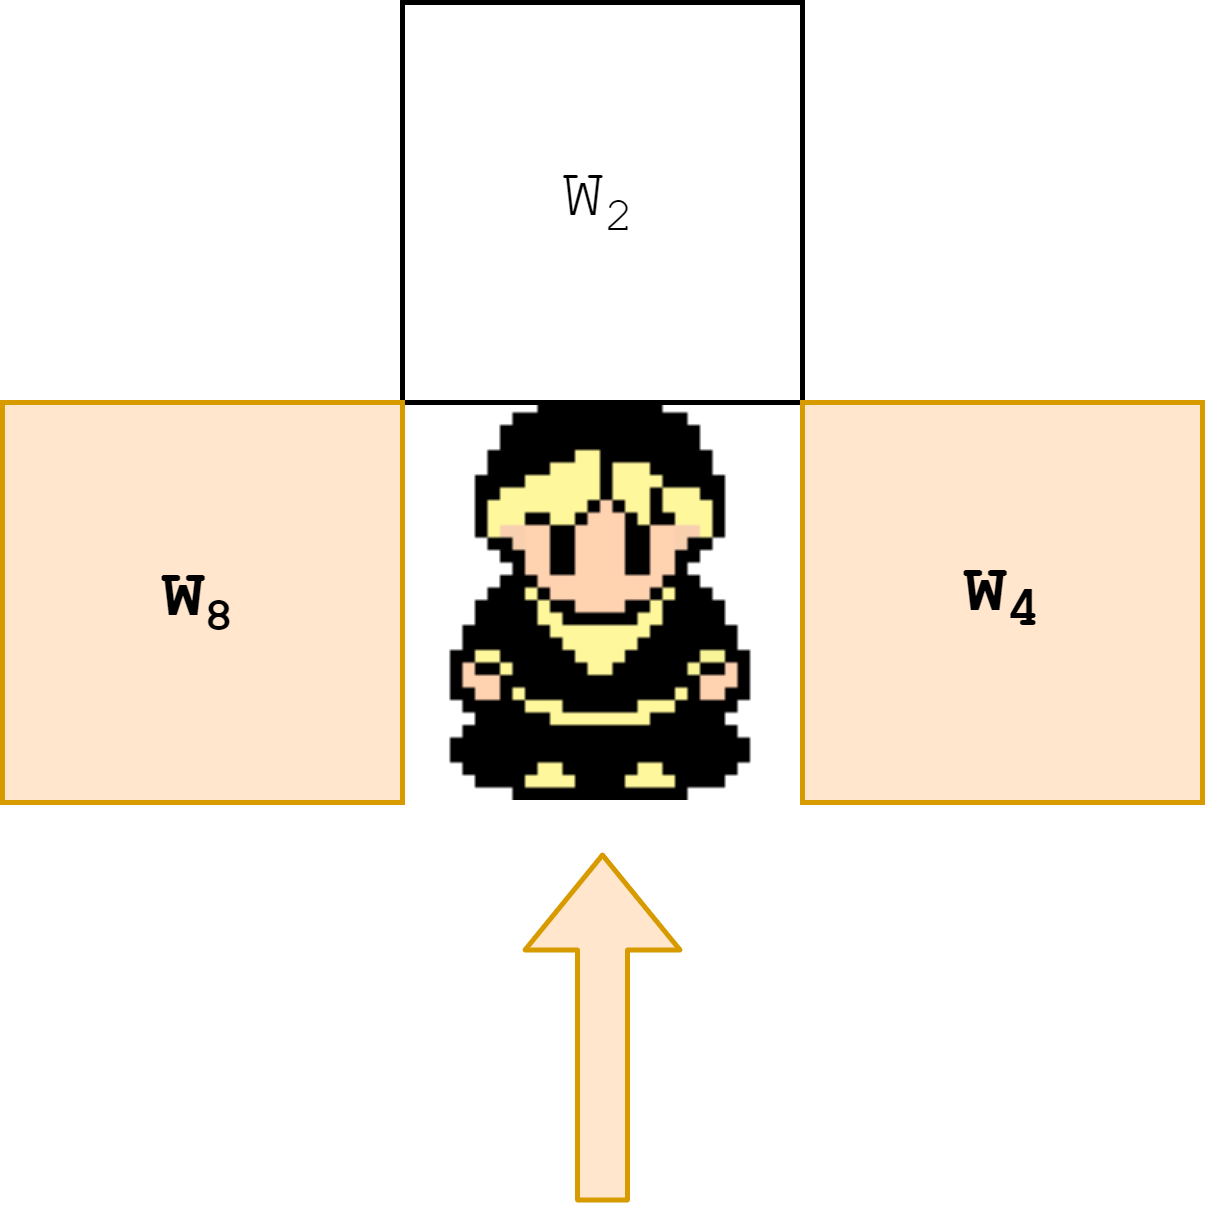
\includegraphics[width=.3\columnwidth]{seguir_norte}}\hspace{1em}
  \subfloat[Pasillo estrecho este]{%
    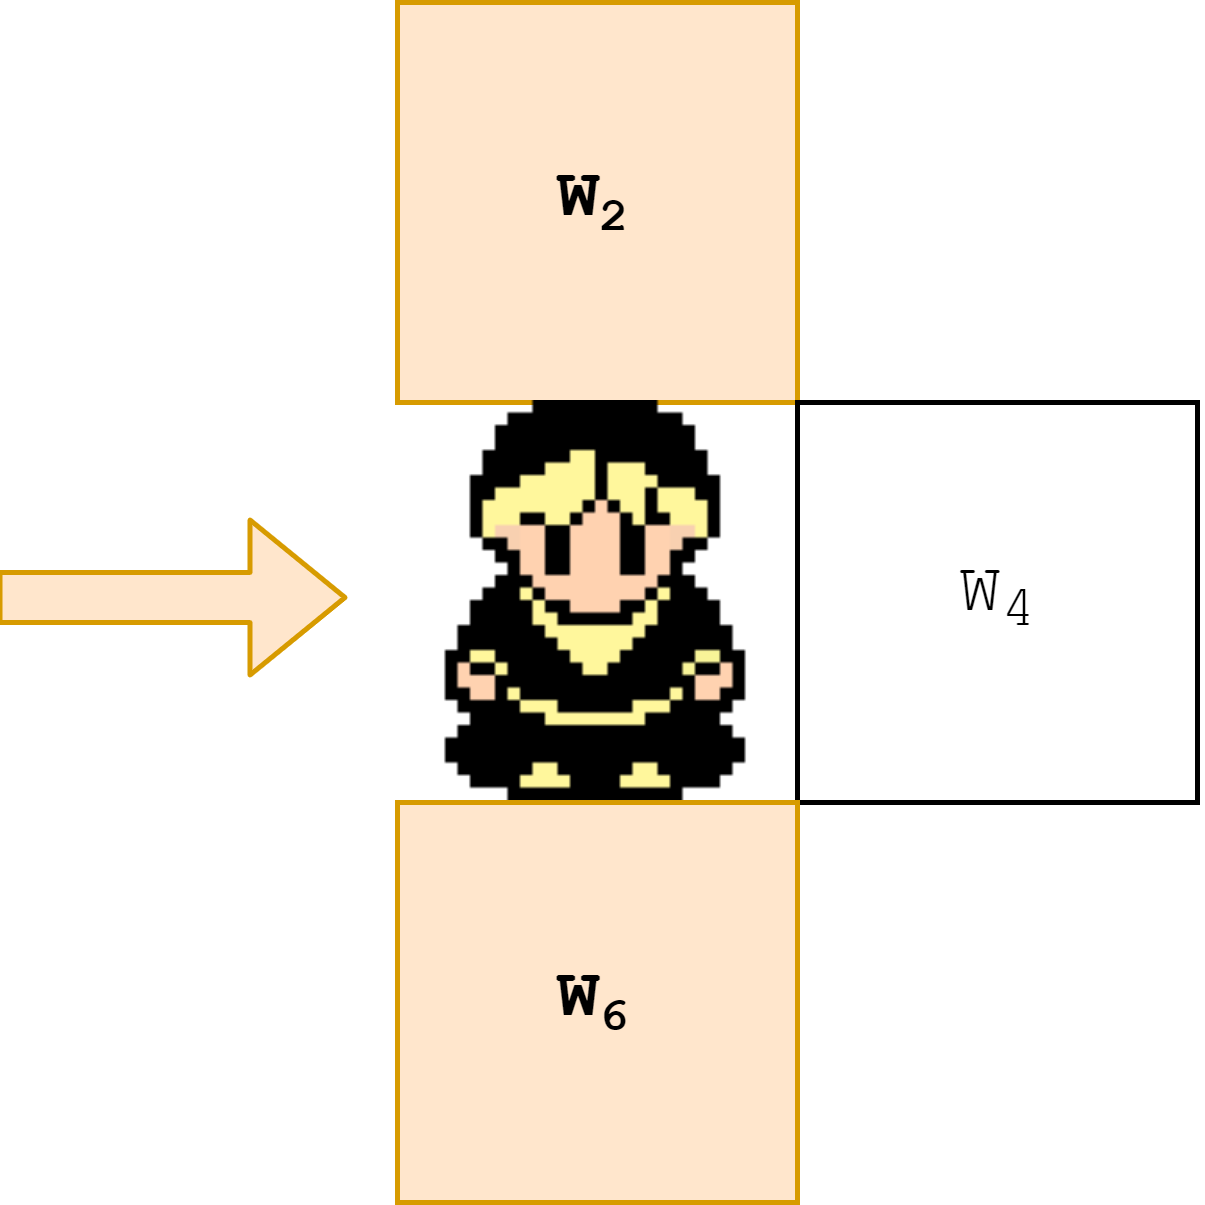
\includegraphics[width=.3\columnwidth]{seguir_este}}\\
  \subfloat[Pasillo estrecho sur]{%
    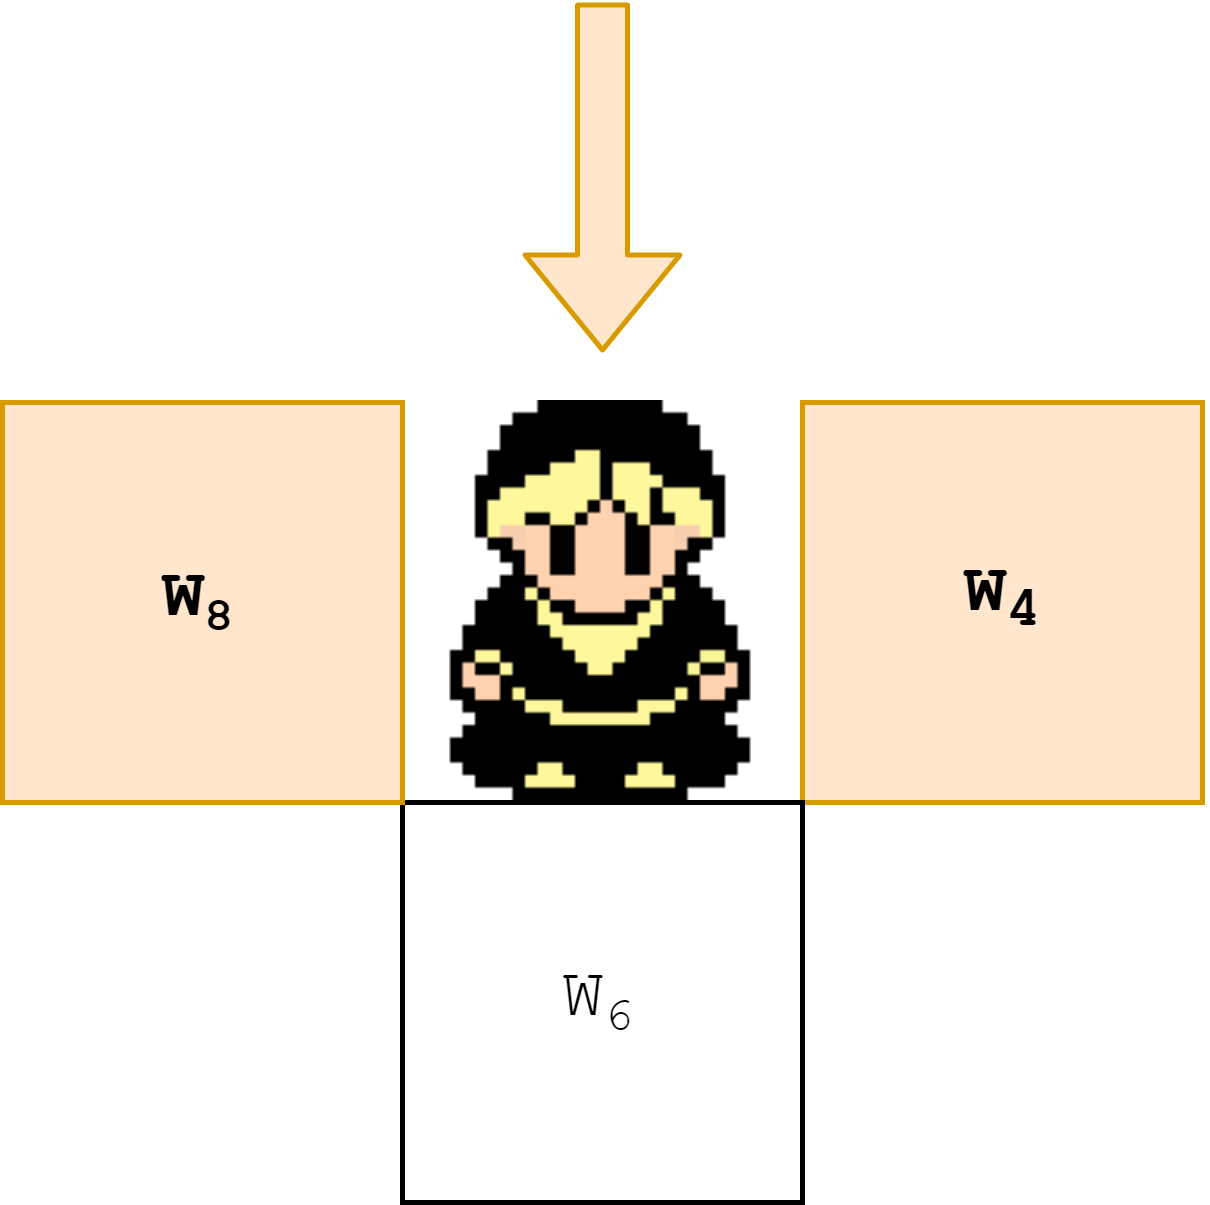
\includegraphics[width=.3\columnwidth]{seguir_sud}}\hspace{1em}
  \subfloat[Pasillo estrecho oeste]{%
    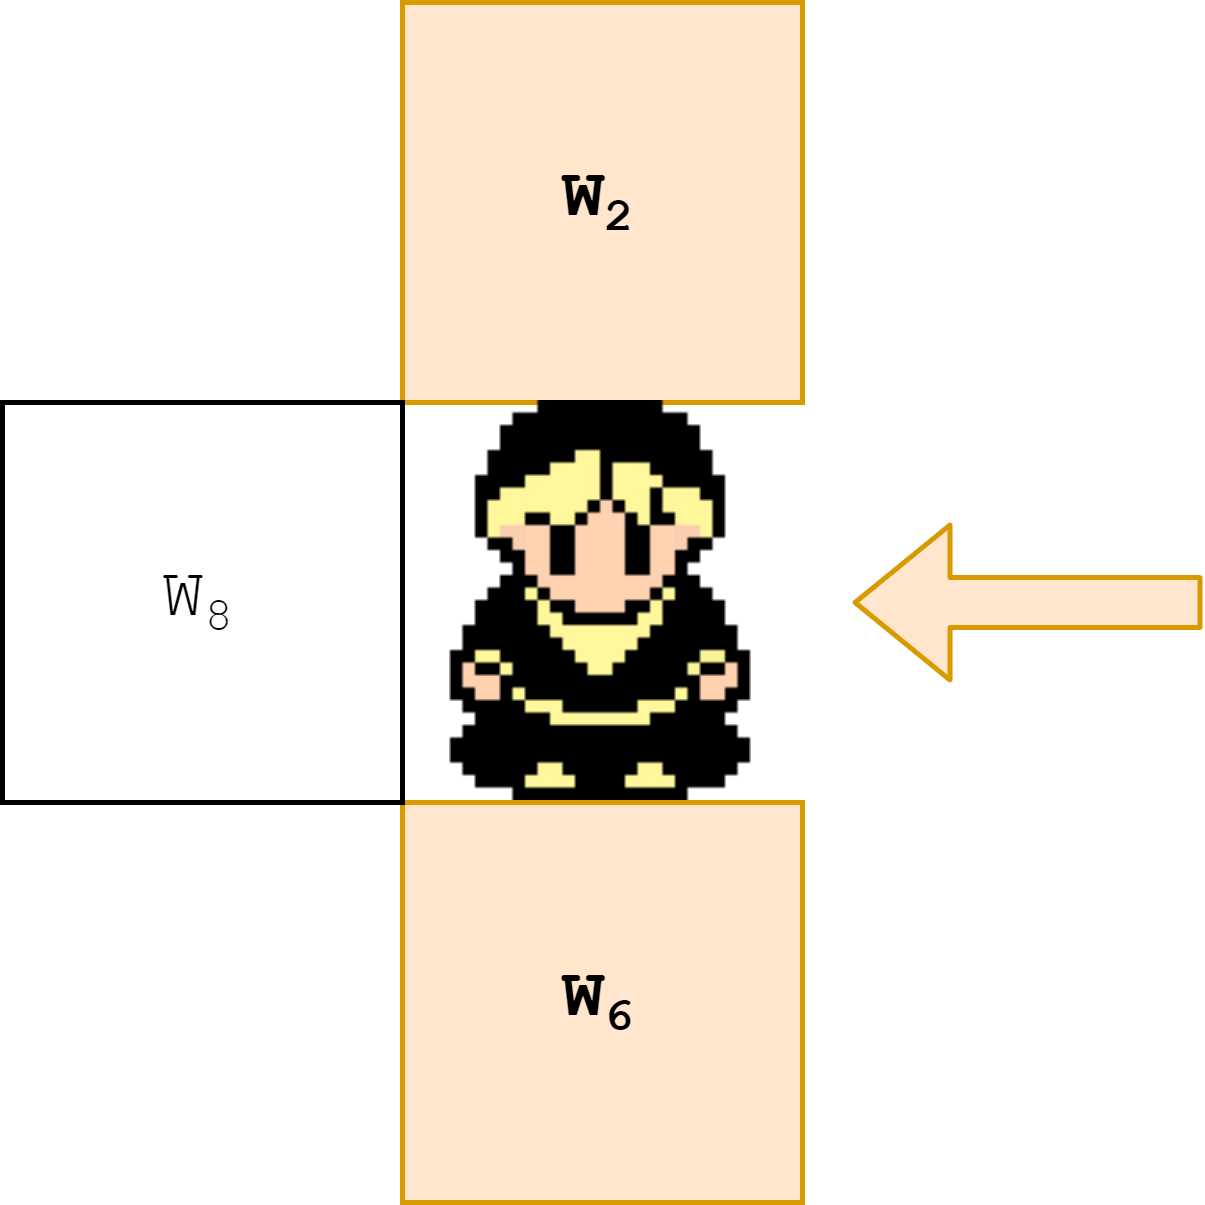
\includegraphics[width=.3\columnwidth]{seguir_oeste}}
  \caption{Casos de recorrido de un pasillo estrecho}\label{fig:seguir_pasillo}
\end{figure}

\FloatBarrier

Las reglas de estos casos son las siguientes:

\begin{itemize}
    \item \emph{$A^{t-1} = Norte \land W_{4} \land W_{8} \land \neg W_{2} \longrightarrow A = Norte $}
    \item \emph{$A^{t-1} = Este \land W_{2} \land W_{6} \land \neg W_{4} \longrightarrow A = Este $}
    \item \emph{$A^{t-1} = Sur \land W_{4} \land W_{8} \land \neg W_{6} \longrightarrow A = Sur $}
    \item \emph{$A^{t-1} = Oeste \land W_{2} \land W_{6} \land \neg W_{8} \longrightarrow A = Oeste $}
\end{itemize}

Con estas reglas, el agente detecta si está en un pasillo estrecho y comprueba si puede seguir realizando la acción anterior (\emph{$A^{t-1}$}).

Las reglas también están ordenadas según su prioridad de ejecución, ya que el agente realiza las acciones en sentido horario.

\subsection{Casos normales}
Las reglas de casos normales se realizan cuando todas las reglas anteriores no se cumplen. Estos casos se dan cuando el agente está recorriendo el entorno en un parte donde no hay no pasillos estrechos o la salido de uno. Además, estas reglas permiten girar al agente en el caso de que se haya encontrado con el final de un pasillo estrecho.

El agente identifica estos casos de la siguiente forma:
\begin{itemize}
    \item En la casilla \emph{$W_{2}$} hay una pared y la casilla \emph{$W_{4}$} está libre. En este caso el agente sabe que debe ir hacia el \emph{Este}.
    
    \item En las casilla \emph{$W_{4}$} hay una pared y la casilla \emph{$W_{6}$} está libre. En este caso el agente sabe que debe ir hacia el \emph{Sur}.
    
    \item En las casilla \emph{$W_{6}$} hay una pared y \emph{$W_{8}$} está libre. En este caso el agente sabe que debe ir hacia el \emph{Oeste}.
    
    \item En las casilla \emph{$W_{8}$} hay una pared y \emph{$W_{2}$} está libre. En este caso el agente sabe que debe ir hacia el \emph{Norte}.
\end{itemize}

\begin{figure}[htb]
\centering
  \subfloat[Este libre]{%
    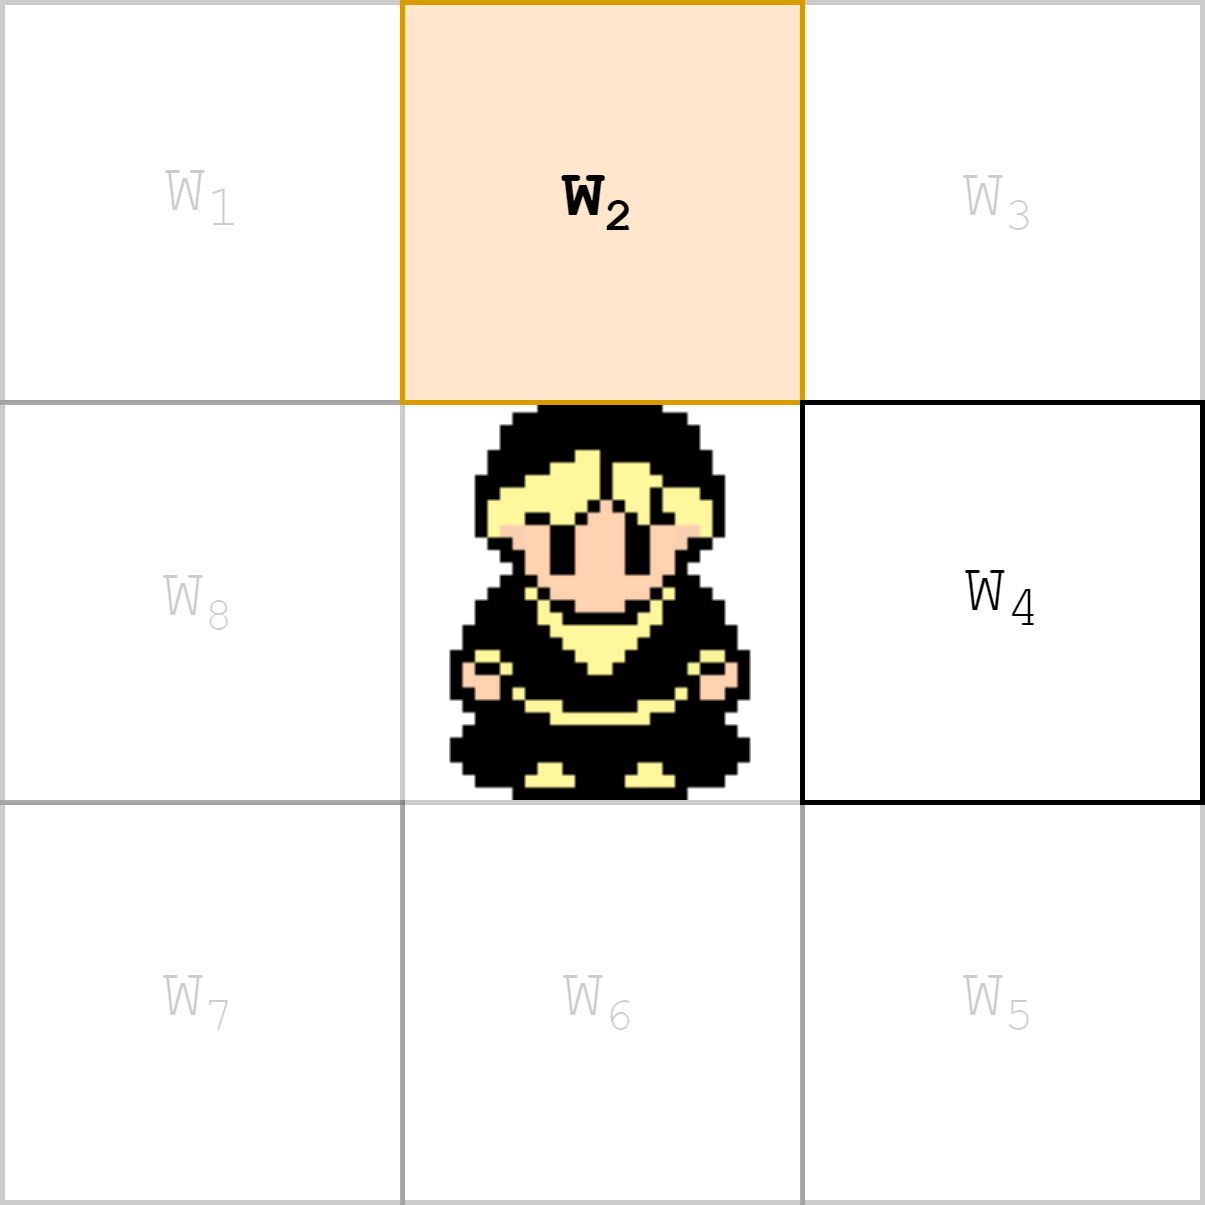
\includegraphics[width=.3\columnwidth]{pared_norte}}\hspace{1em}
  \subfloat[Sur libre]{%
    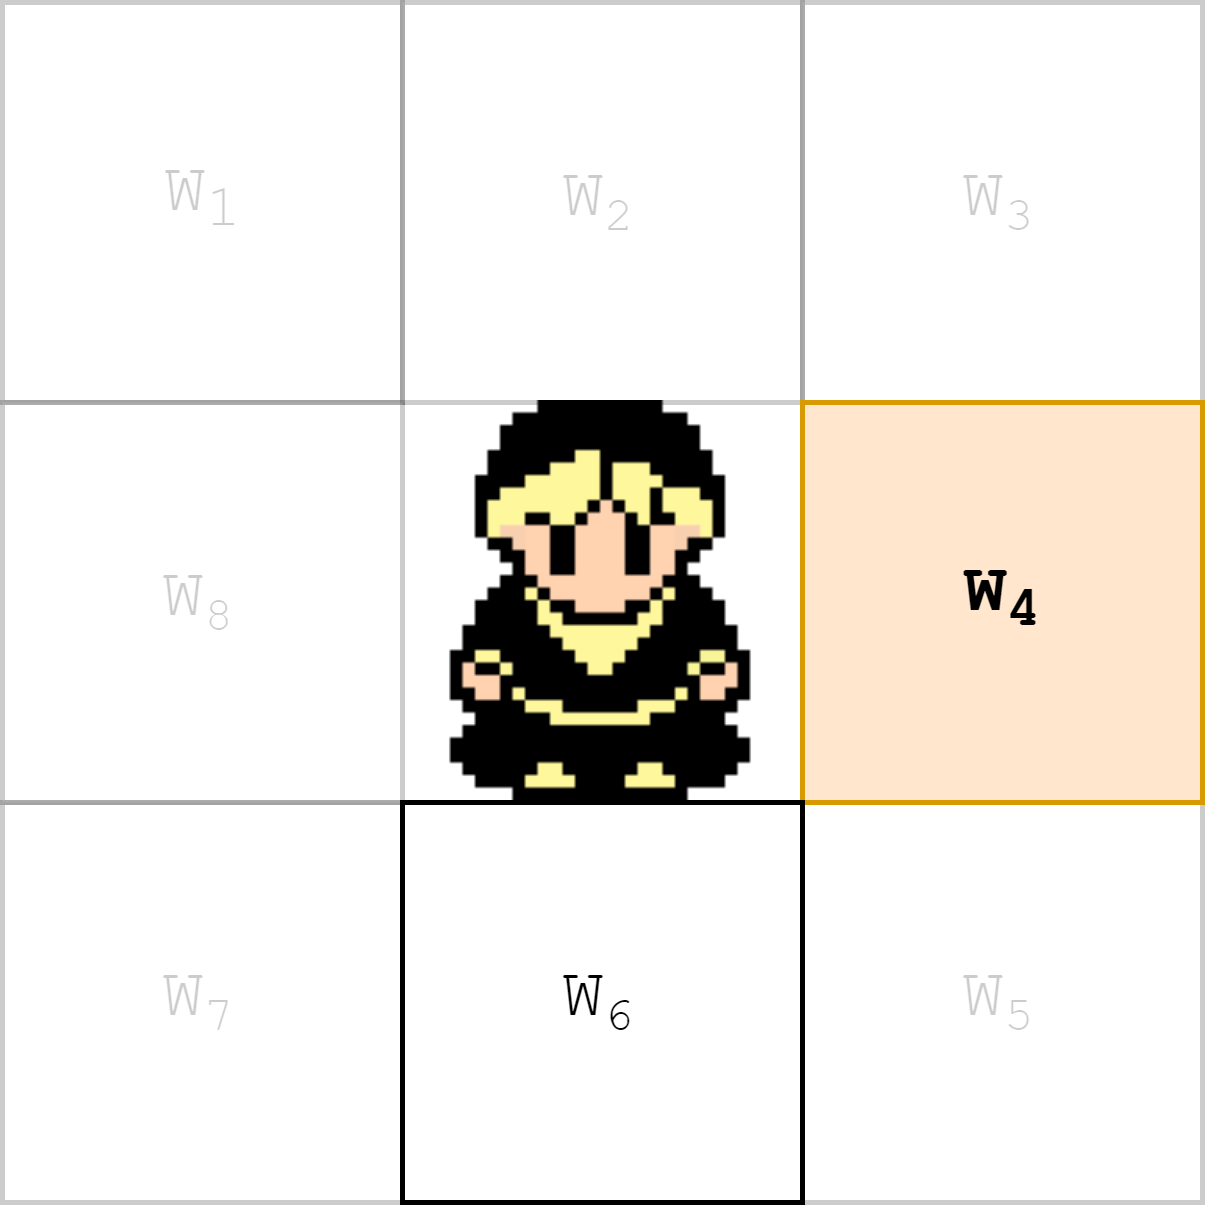
\includegraphics[width=.3\columnwidth]{pared_este}}\\
  \subfloat[Oeste libre]{%
    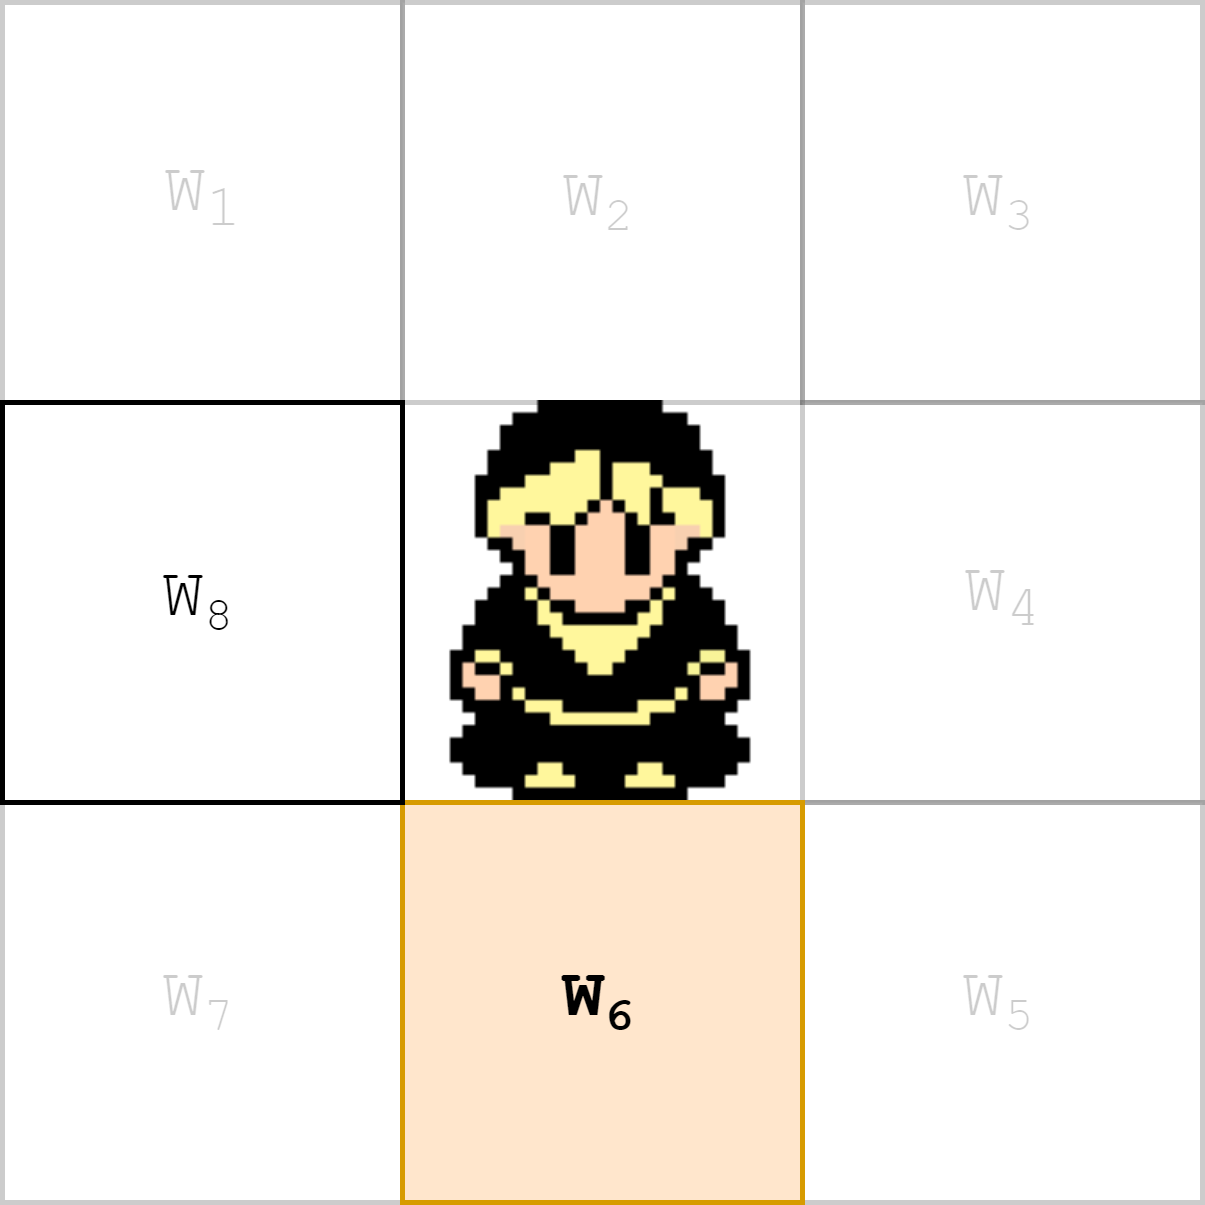
\includegraphics[width=.3\columnwidth]{pared_sud}}\hspace{1em}
  \subfloat[Norte libre]{%
    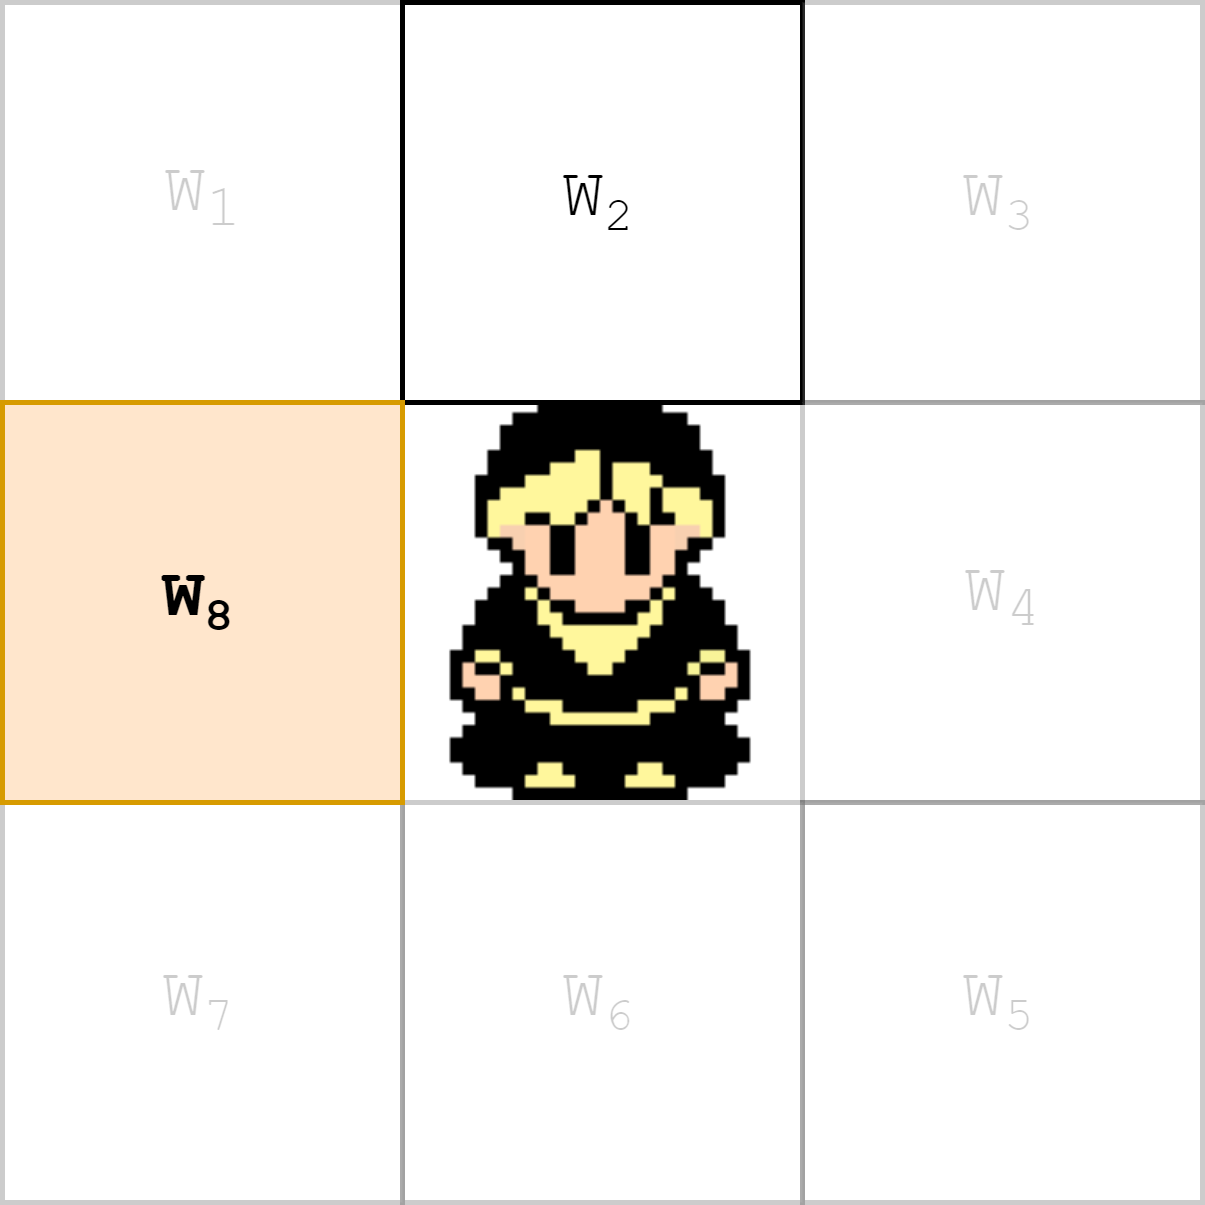
\includegraphics[width=.3\columnwidth]{pared_oeste}}
  \caption{Casos normales (agente pegado a una pared)}\label{fig:seguir_pared}
\end{figure}

\FloatBarrier

Estos casos se dan cuando el agente este en contacto con las paredes, pero también puede ser que el agente haya dejado de seguir una pared. Estos casos son los siguientes:

\begin{itemize}
    \item En la casilla \emph{$W_{1}$} hay una pared. En este caso el agente irá hacia el \emph{Norte}.
    \item En la casilla \emph{$W_{3}$} hay una pared. En este caso el agente irá hacia el \emph{Este}.
    \item En la casilla \emph{$W_{5}$} hay una pared. En este caso el agente irá hacia el \emph{Sur}.
    \item En la casilla \emph{$W_{7}$} hay una pared. En este caso el agente irá hacia el \emph{Oeste}.
\end{itemize}

En cada caso descrito, el agente está seguro de que seguirá una pared siempre. Pero se puede dar que el agente se encuentre en un entorno sin ninguna pared o que en la posición donde ha aparecido no hay ninguna pared a su alrededor. Por eso hay que establecer un acción que se realizará cuando se da el caso anterior. Esta acción es que al gente siempre vaya hacia el \emph{Norte}.

Con estos casos, podemos establecer las siguientes reglas:

\begin{itemize}
    \item \emph{$W_{2} \land \neg W_{4} \longrightarrow A = Este$}
    \item \emph{$W_{4} \land \neg W_{6} \longrightarrow A = Sur$}
    \item \emph{$W_{6} \land \neg W_{8} \longrightarrow A = Oeste$}
    \item \emph{$W_{8} \land \neg W_{2} \longrightarrow A = Norte$}
    \item \emph{$W_{1} \longrightarrow A = Norte$}
    \item \emph{$W_{3} \longrightarrow A = Este$}
    \item \emph{$W_{5} \longrightarrow A = Sur$}
    \item \emph{$W_{7} \longrightarrow A = Oeste$}
    \item \emph{$\longrightarrow A = Norte$}
\end{itemize}

Juntado todas las reglas anteriores, esta sería la base de reglas que utilizaría el agente para conseguir su meta:

\begin{itemize}
    \item \emph{$A^{t-1} = Oeste \land W_{5} \land \neg W_{6} \longrightarrow A = Sur $}
    \item \emph{$A^{t-1} = Sur \land W_{3} \land \neg W_{4} \longrightarrow A = Este $}
    \item \emph{$A^{t-1} = Este \land W_{1} \land \neg W_{2} \longrightarrow A = Norte $}
    \item \emph{$A^{t-1} = Norte \land W_{7} \land \neg W_{8} \longrightarrow A = Oeste $}
    \item \emph{$A^{t-1} = Norte \land W_{4} \land W_{8} \land \neg W_{2} \longrightarrow A = Norte $}
    \item \emph{$A^{t-1} = Este \land W_{2} \land W_{6} \land \neg W_{4} \longrightarrow A = Este $}
    \item \emph{$A^{t-1} = Sur \land W_{4} \land W_{8} \land \neg W_{6} \longrightarrow A = Sur $}
    \item \emph{$A^{t-1} = Oeste \land W_{2} \land W_{6} \land \neg W_{8} \longrightarrow A = Oeste $}
    \item \emph{$W_{2} \land \neg W_{4} \longrightarrow A = Este$}
    \item \emph{$W_{4} \land \neg W_{6} \longrightarrow A = Sur$}
    \item \emph{$W_{6} \land \neg W_{8} \longrightarrow A = Oeste$}
    \item \emph{$W_{8} \land \neg W_{2} \longrightarrow A = Norte$}
    \item \emph{$W_{1} \longrightarrow A = Norte$}
    \item \emph{$W_{3} \longrightarrow A = Este$}
    \item \emph{$W_{5} \longrightarrow A = Sur$}
    \item \emph{$W_{7} \longrightarrow A = Oeste$}
    \item \emph{$\longrightarrow A = Norte$}
\end{itemize}